\subsection{Blockchain}
\label{sec:sota_blockchain}
    Eine Blockchain ist in ihrer Essenz eine immer länger werdende, unveränderbare, öffentliche Kette von Transaktionen, die dezentral gespeichert wird (s. \fref{fig:bc_highlvl}). 
    \smallskip
    \todo[color=yellow]{Transaktionen in m umbenennen (zu Hause}
    \begin{figure}[H]
    	\centering
    	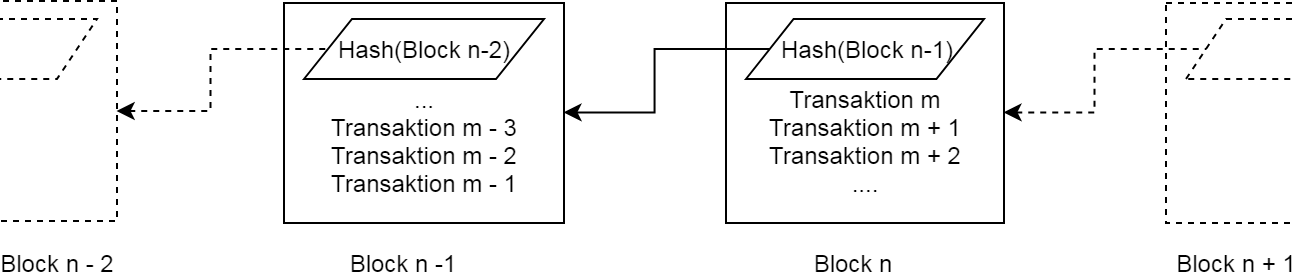
\includegraphics[width=\textwidth]{graphics/bc_highlvl.png}
    	\caption[Abstrakte Darstellung einer Blockchain]{Abstrakte Darstellung einer Blockchain. Jeder neu hinzugefügte Block (hier immer rechts angehängt) enthält eine Referenz auf den Vorigen mittels dessen Hashwert.}
    	\label{fig:bc_highlvl}
    \end{figure}
    \noindent Erstmals 2008 von Satoshi Nakamoto, ursprünglich als Peer-to-Peer Electronic Cash System ,,Bitcoin``
    \!\footnote{Heute werden Bitcoin, Ether, Ripple und andere als digitale Zahlungsmittel als sogennante Kryptowährung bezeichnet} 
    erfunden, erregte die Technologie aufgrund ihrer Eigenschaften wie ihres dezentralen, anonymen Konzepts schnell Aufmerksamkeit. 
    Bitcoin ist die erste populäre digitale Währung, die ohne zentrale Autorität wie beispielsweise einer \gls{ttp} das in \fref{sec:sota_doublespend} vorgestellte Double-Spending Problem lösen sollte\cite{Nakamoto2008}. 
    Übertragen auf Bitcoin bedeutet es, dass ein Empfänger einer Transaktion sichergehen können muss, dass der vorige Besitzer den Bitcoin oder den Bruchteil dessen vorher nicht schon einmal erfolgreich an einen anderen Empfänger gesendet hat.
    Dies wird mittels kryptographischem Beweis, welcher in \fref{sec:sota_blockchain_consensus} genauer betrachtet wird, anstatt des laut \citeauthor{Nakamoto2008} vorstellten mangelhaften Modells dker \gls{ttp}, welche stets einen Single Point of Failure
    \!\footnote{Ein Single Point of Failure stellt beipsielsweise eine Bank im Zahlungsverkehr dar.
    Fällt die Bank beispsielsweise aus irgendeinem Grund aus oder wird kompromittiert, haben deren Kunden keine Möglichkeit mehr (sicher) Überweisungen auszuführen und zu empfangen.}
    darstellt, gelöst. 
    Das Konzept ermöglicht es somit zwei Entitäten, auch, wenn sie sich gegenseitig nicht vertrauen, ohne vermittelnde Person oder Organisation eine sichere (im Sinne der Vertraulichkeit) direkte Transaktionen miteinander durchzuführen, welche auch im Nachhinein nicht mehr verändert werden können.\cite{Christidis2016}
    
    \subsubsection{Einführung in das Konzept}
    \label{sec:sota_blockchain_introduction}
    Grundlegend ist die Blockchain eine verteilte Datenstruktur, die zwischen den Mitgliedern eines Netzwerkes repliziert und geteilt wird\cite{Christidis2016}.
    Die Blockchain beinhaltet das maßgebliche ,,Hauptbuch`` (im Englischen ,,Ledger`` genannt) mit allen vergangenen Transaktionen, ein Log, dessen Einträge mit Zeitstempeln jeweils zu unterschiedlichen Blöcken zusammengefasst werden. 
    Alle vergangenen Transaktionen in der Reihenfolge ihres Auftretens sind für alle Teilnehmer einsehbar\cite{Nakamoto2008}.
    \medskip\\
    Nutzer nehmen an dem Netzwerk über Knoten teil, wobei ein Knoten auch für mehrere Nutzer einen Zugang bieten kann(s. \fref{fig:bc_network}). 
    Knoten des Netzwerkes speichern stets eine eigene Kopie der Blockchain.
    Jeder Nutzer interagiert mit dem Netzwerk mittels eines Paares von öffentlichem und privatem Schlüssel, wobei der Öffentliche oder dessen Hashwert zur Adressierung und der Private zur Signierung von Transaktionen des Nutzers verwendet wird.\cite{Christidis2016}
    \begin{figure}[H]
    	\centering
    	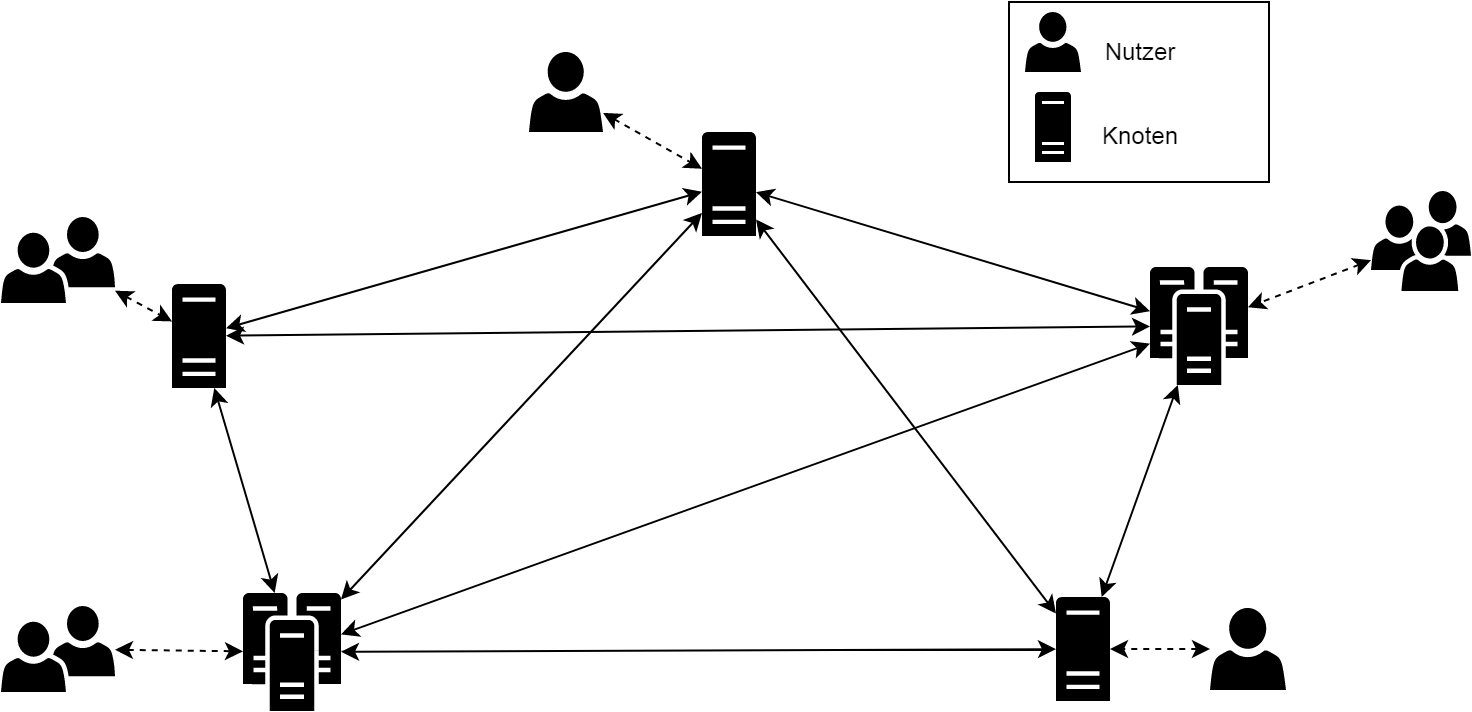
\includegraphics[width=\textwidth]{graphics/BCNetwork.png}
    	\caption[Blockchain-Netzwerk]{Blockchain-Netzwerk}
    	\label{fig:bc_network}
    \end{figure}
    
    Zunächst wurde mit digitalen Coins gehandelt, welche einer in Form einer Kette digitaler Signaturen modelliert wurden\cite{Nakamoto2008}.
    In anderen Anwendungsbereichen außerhalb des Bereiches der Kryptowährungen wird von generalisierten Assets gesprochen.
    Der aktuelle Zustand (,,World View`` genannt) ergibt sich also durch das Zurückverfolgen der einzelnen Transaktionen in der Blockchain. 
    Es wird also kein aktueller Stand, welcher Teilnehmer des Netzwerks was und wie viel besitzt, gespeichert.\cite{Christidis2016}
    
    \subsubsection{Transaktionen}
    \label{sec:sota_blockchain_trx}
    In einer Blockchain werden Aktivitäten von Nutzern in Form von Transaktionen repräsentiert. 
    
    Tätigt ein Nutzer eine Transaktion \lstinline{X}, so signiert er diese mit seinem privaten Schlüssel, der Knoten, über welchen der Nutzer mit dem Netzwerk interagiert, validiert diese, sammelt diese und verteilt die valide Transaktion an die nächsten Nachbarn
    \!\footnote{Nächste Nachbarn sind jene Knoten, die einen Sprung im \gls{p2p}-Netzwerk voneinander entfernt sind.}.
    Die Nachbarn überprüfen die Transaktion ebenfalls auf deren Validität und verbreiten diese wiederrum an ihre nächsten Nachbarn. 
    Schlussendlich kennen eine Vielzahl von Knoten im Netzwerk die Transaktion \lstinline{X}. 
    
    Im sogenannten ,,Mining``-Prozess, der wiederholt wird, werden valide Transaktionen, die innerhalb eines im Voraus abgestimmten Zeitintervalls gesammelt wurden, zeitlich geordnet, zu einem mit Zeitstempel versehenem ,,Candidate``-Block zusammengefügt und wieder im Netzwerk verbreitet. 
    Andere Knoten im Netzwerk stellen sicher, dass der neue Block valide Transaktionen enthält und den richtigen Hash des vorigen Blocks in der Kette enthält. 
    Bei erfolgreicher Validierung hängen die Knoten den Block jeweils an ihre Kopie der Kette an, übernehmen die darin enhaltenen Transaktionen und aktualisieren somit den aktuellen Zustand. 
    Sollte innerhalb des Mining-Prozesses eine Validierung fehlschlagen, wird der ganze Block verworfen.
    
    Der Knoten, der diesen Prozess ausführt wird Miner genannt und von der Auswahl des Knotens und Konsensmechanismus abhängig und unter Umständen in der gleichen Situation unterschiedlich.\cite{Christidis2016}
    
    \begin{figure}[H]
    	\centering
    	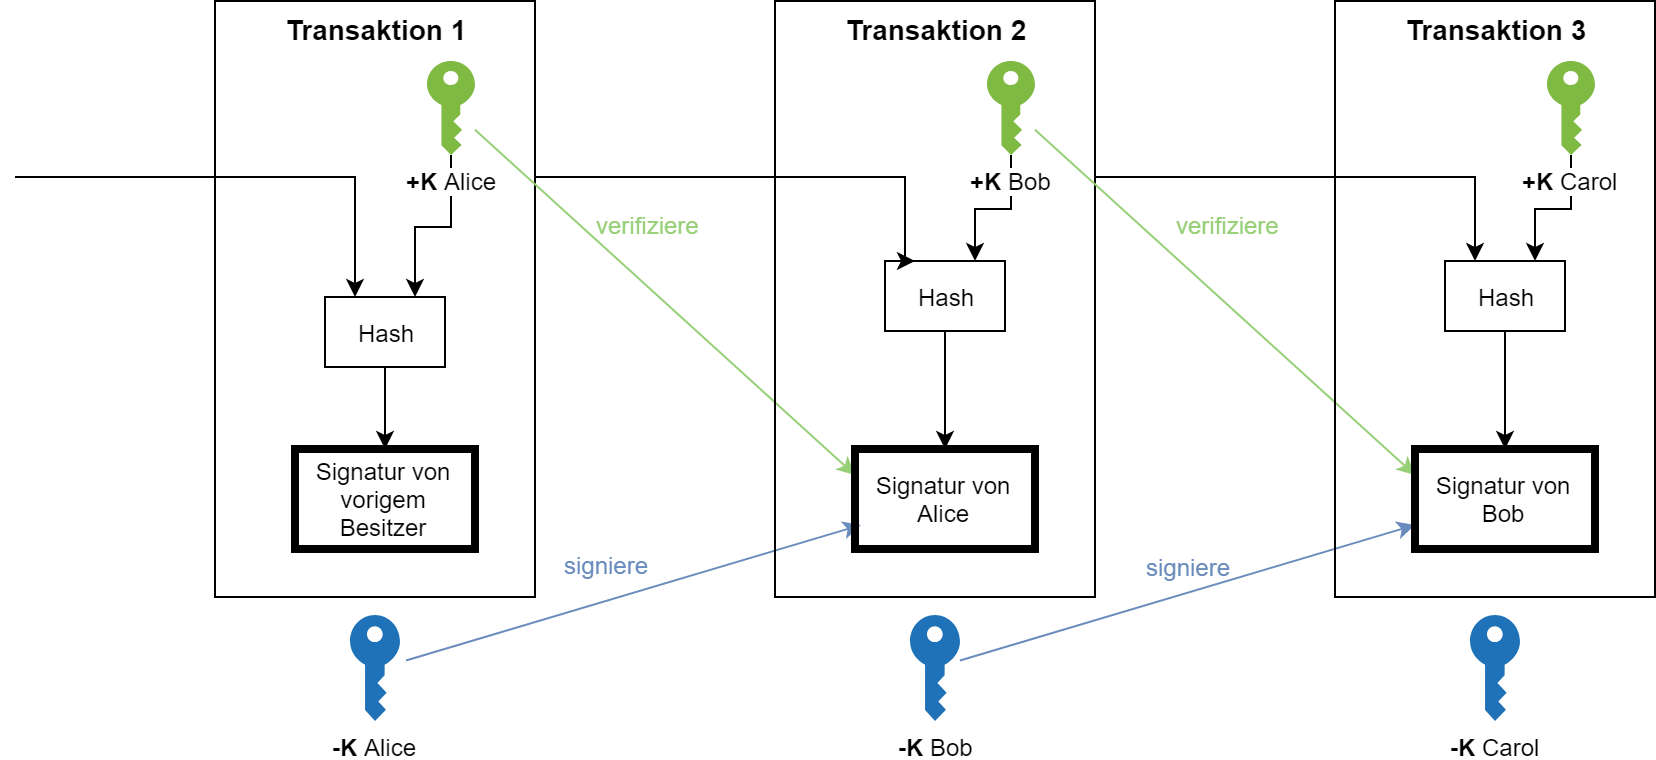
\includegraphics[width=\textwidth]{graphics/transaction.png}
    	\caption[Kette digitaler Signaturen]{Kette digitaler Signaturen\cite{Nakamoto2008}. \lstinline{+K} stellt dabei den öffentlichen und \lstinline{-K} den privaten Schlüssel dar.}
    	\label{fig:txio}
    \end{figure}
    
    Wie in \fref{fig:txio} dargestellt, werden Assets von einem Versender zu einem Empfänger transferiert, in dem der Sender einen Hash der vorigen Transaktion und den öffentlichen Schlüssel des Empfängers mit seinem eigenen privaten Schlüssel digital signiert und diese Hash dann am Ende des Assets anfügt.
    Der Empfänger, sowie alle Teilnehmer des Netzwerkes können den Besitz des Assets über die Kette der digitalen Signaturen zurückverfolgen.
    Transaktionen können zudem mehrere Ein- und Ausgaben haben.\cite{Nakamoto2008}
    
    Getätigte Transaktionen sollen nicht mehr rückgängig gemacht werden können.
    Erreicht wird dies, indem die Rückrechnung des Beweises rechnerisch zu aufwändig sein soll\cite{Nakamoto2008}.
    Somit wird der Verkäufer vor Täuschung geschützt und Treuhandmechanismen können einfach implementiert werden\cite{Nakamoto2008}.  
    \medskip\\
    Wie in \fref{fig:txio} dargestellt, werden Assets von einem Versender zu einem Empfänger transferiert, in dem der Sender einen Hash der vorigen Transaktion und den öffentlichen Schlüssel des Empfängers mit seinem eigenen privaten Schlüssel digital signiert und diese Hash dann am Ende des Assets anfügt.
    Transaktionen können zudem mehrere Ein- und Ausgaben haben\cite{Nakamoto2008}.
    
    Der Empfänger, sowie alle Teilnehmer des Netzwerkes können den Besitz des Assets über die Kette der digitalen Signaturen zurückverfolgen\cite{Nakamoto2008}.
	
	\subsubsection{Typen}
    \label{sec:sota_blockchain_types}
        Mit einer Blockchain können auch je nach Anwendungsszenario, außer Kryptowährungen, andere (als Token  repräsentierte) Waren oder Assets wie Güter im Supply Chain Management\cite{Underwood2016}, Identitäten zur Zugangskontrolle\cite{Kshetri2017} oder Proof of Ownership digitaler Rechte\cite{Wuest2017} gespeichert und gehandelt werden. 
        Unterschiedliche Anwendungen haben auch verschiedene Anforderungen an die Blockchain selbst. 
        Bei Anwendungen wie Supply Chain Management rückt beispielsweise der Aspekt ohne \gls{ttp} auszukommen eher in den Hintergrund. 
        Wichtig ist dort eher die Unveränderbareit und Nachverfolgbarkeit von Transaktionen in der Blockchain, die dabei helfen den Weg von Gütern von Start zum Ziel nachvollzeihbar zu machen. 
        Zur Zeit haben sich unterschiedliche Typen einer Blockchain herauskristallisiert, welche je nach Autor teilweise verschieden bezeichnet werden.
        Nach \cite{Wuest2017,Christidis2016,Buterin2015,Vukolic2017} wird in unterschiedliche Typen unterschieden:
        \begin{enumerate}[noitemsep]
            \item \textbf{public/permissionless}, Beispiele: Bitcoin, Ethereum\\
                Jeder kann zu einem beliebigen Zeitpunkt dem Netzwerk beitreten oder es verlassen und kann sowohl lesen, als auch schreiben und an dem Prozess der Konsensfindung teilnehmen. 
                Es existiert keine zentrale Autorität, welche die Mitgliedschaft im Netzwerk verwaltet und beispielsweise Teilnehmer, die aufgrund ihrer Handlungen ausgeschlossen werden sollen, verbannen könnte. 
            \item \textbf{public/permissioned} (auch Konsortium genannt), Beispiele: Microsoft Azure Coco\\
                Eine Gruppe von Organisationen oder eine Menge ausgeswählter Knoten reguliert und verwaltet eine Liste der Teilnehmer des Netzwerkes und deren Berechtigungen (lesen/schreiben), verifiziert Transaktionen und vollzieht den Miningprozess. 
                Somit können die einzelnen Transaktionen schneller überprüft, an die Blockchain angehängt und somit ausgeführt werden als bei einer öffentlichen Blockchain.
            \item \textbf{private/permissioned}, Beispiele: Hyperledger Fabric\\
                Ähnlich den public/permissioned Blockchains werden auch private von mindestens einer zentralen Autorität verwaltet, welche sich innerhalb einer einzelnen Organisation befindet.
                \todo[color=yellow]{etwas mehr beschreiben?}
        \end{enumerate}
	
    \subsubsection{Konsens und Sicherheit}
    \label{sec:sota_blockchain_consensus}
        Um Transaktionen selbst zu validieren, deren Reihenfolge im nächsten Block zu bestimmen und Mining-Blöcke auszuwählen zu können wird von allen Teilnehmern des Netzwerkes ein gemeinsamer Konsens vorausgesetzt. 
        Ist dies nicht der Fall können, wie in \fref{fig:bc_forks} dargestellt, unterschiedliche Ketten (,,Forks`` genannt) innerhalb der jeweiligen Kopien der Blockchain auf den einzelnen Knoten entsehen. 
        
        \begin{figure}[H]
        	\centering
        	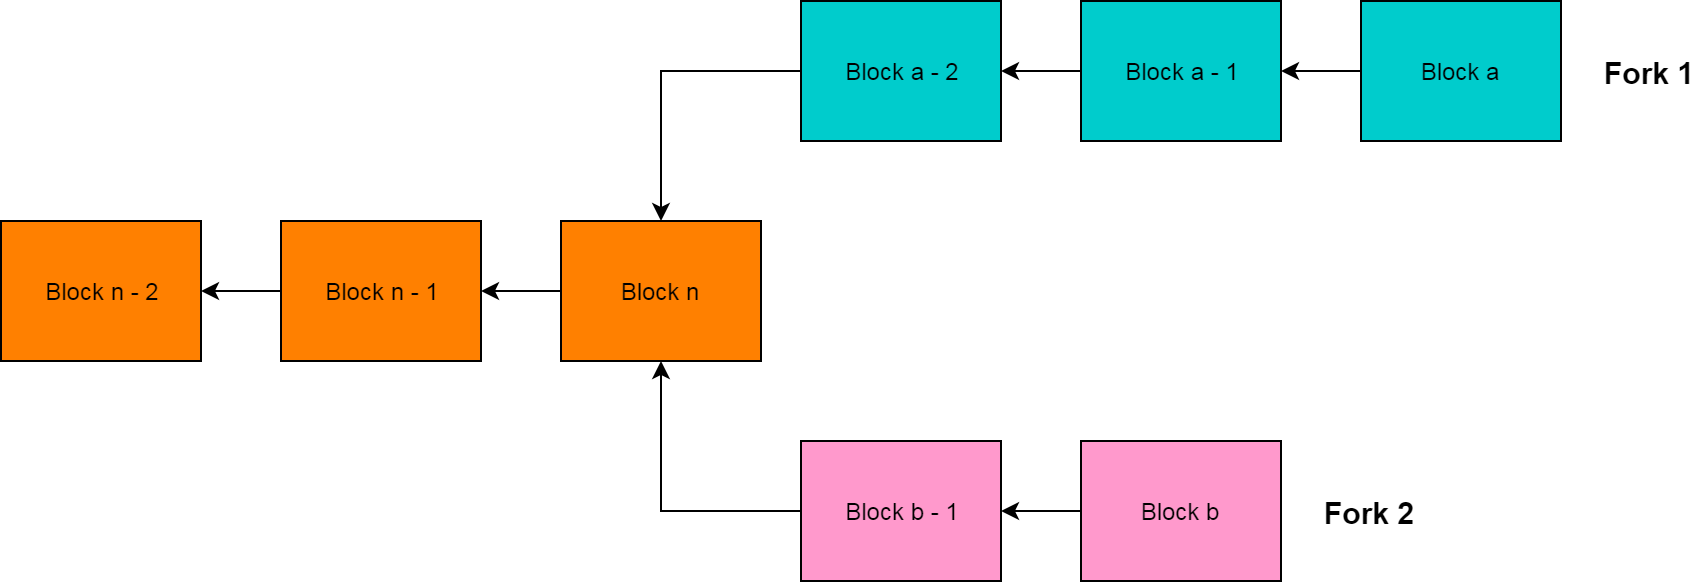
\includegraphics[width=\textwidth]{graphics/BCForks.png}
        	\caption[Blockchain mit Forks]{Blockchain mit zwei Forks}
        	\label{fig:bc_forks}
        \end{figure}
        \noindent Ideal wäre es, wenn alle validierenden Knoten des Netzwerkes abstimmen und die Mehrheit über die Reihenflolge der Transaktionen für den nächsten Block entscheidet.\cite{Christidis2016} 
        Aufgrund der Gefahr eines ,,Sybil-Angriffs``\cite{Trifa2014}
        \!\footnote{Bei einem ,,Sybil-Angriff`` erlangt ein Angreifer mehr Einfluss auf die Abstimmung, indem er entweder zusätzliche Nutzeridentitäten für sich selbst erstellt oder mehrere Knoten kontrolliert.
        } ist dies jedoch unzumutbar.
        Um diese Gefahr zu umgehen werden unterschiedliche Methoden angewendet, von denen einige Ausgewählte kurz erläutert werden:\cite{Christidis2016}
        \smallskip\\
        Bei Bitcoin wird ein sogenannnter \gls{pow} verwendet. 
        Das Mining wird rechnerisch ,,teuer`` gemacht, indem vorausgesetzt wird, dass ein minender Knoten eine richtige Zufallszahl (genannt ,,Nonce``) mit variablem Schwierigkeitsgrad und mit bestimmten Eigenschaften berechnet und mit einer bestimmten Anzahl Bitcoins belohnt wird. 
        Da bei der Berechnung kryptographische Hashfunktionen verwerndet werden, kann das Ergebnis durch die anderen Knoten einfach verifiziert werden. 
        Diese Zahl kann jeder Knoten im Netzwerk berechnenn, sodass die explizite Auswahl des Miners entfällt. 
        Der Candidate-Block jenes Knotens, der den Nonce findet, wird an die Blockchain angehängt. 
        Sollten Forks entstehen, wird der Fork verwendet, in der der meiste Rechenaufwand steckt. 
        Oft sind dies entweder der längste Fork oder der Fork, mit dem höchsten Schwierigkeitsgrad.\cite{Christidis2016,Nakamoto2008}
        \smallskip\\
        Alternativ kann ein \gls{pos} verwendet werden, welcher bedeutend weniger Rechenaufwand erfordert. 
        Dabei senden sich Besitzer selbst eine bestimmte Anzahl an Coins und addieren einen vordefinieren Prozentsatz als Belohnung. 
        Analog zum \gls{pow} wird ein Hashwert, entweder größer oder kleiner als ein gesuchter Wert ist berechnet, wobei die Schwierigkeit der Berechnung (umgekehrt proportional zum Alter der Coins) individuell festgelegt wird. 
        Der Hashwert wird aus statischen Daten, ausgenommen des Zeitstempels, berechnet, sodass bei jeder Änderung des Zeitstempels eine Chance zum Finden des Hashwertes besteht und die individuelle Rechenleistung der Knoten nur eine minimale Rolle spielt. 
        Wird ein Wert gefunden, so wird die Belohnung an den minenden Knoten ausgeschüttet und das Alter der Coins zurückgesetzt.\cite{Tschorsch2016}
        \medskip\\
        \gls{pow} und \gls{pos} werden vornehmlich in public (permissionless) Netzwerken eingesetzt.
        Für private Blockchains sind sie jedoch eher ungeeignet, da in solchen Netzwerken die Teilnehmer häufig per Whitelist bekannt sind. 
        In solchen Fällen werden Algorithmen wie das Practical \gls{bft} angewendet. Es löst das Problem der byantinischen Generäle
        \!\footnote{TODO
        } in asynchronen Umgebungen. 
        Es schließt ein Protokoll mit drei Phasen ein, sowie der Idee eines Primärknotens, welcher als Block Miner agiert. 
        Der Primärknoten kann über eine ,,View-Change``-Abstimmung geändert werden, falls dieser ausfällt oder sich willkürlich verhält (byzantinischer Fehler).
        Jedoch wird bei diesem Algorithmus davon ausgegangen, dass sich weniger als ein Dittel der Knoten fehlerhaft verhalten.
        \cite{Christidis2016}
    
    \subsubsection{Smart Contracts}
    \label{sec:sota_blockchain_sc}
        Smart Contracts sind Skripte, die innerhalb einer Blockchain gespeichert werden (ähnlich der Stored Procedures eines Relationalen Datenbankmanagementsystems) und agieren autonom. 
        Sie haben eine eigene Adresse und werden angesteuert, indem sie als Empfänger einer Transaktion adressiert werden.
        Die Ausführung passiert unabhängig automatisch und mit vorgegebenem Verhalten auf jedem Knoten des Netzwerks. \cite{Christidis2016}
        \smallskip\\
        Ein Beispiel für einen Smart Contract ist die Überprüfung von Transaktionen. 
        Dabei wird beispielsweise kontrolliert, ob der Sender mindestens die Anzahl an digitalen Token besitzt, die bei der Transaktion an den Empfänger übertragen werden sollen.
    
    \iffalse
    \subsubsection{Sicherheit}
    \label{sec:sota_blockchain_security}
        \begin{itemize}
            \item Users interact with the blockchain via a pair of private/public keys [13]. They use their private key to sign their own transactions, and they are addressable on the network via their public key.2 The use of asymmetric cryptography brings authentication, integrity, and nonrepudiation into the network\cite{Christidis2016}
            \item sonst noch was?
        \end{itemize}
    
    \subsubsection{Identity Management}
    \label{sec:sota_blockchain_identitymgmnt}
        ??
    \fi
